\chapter{Cadre général du projet}
    %\addcontentsline{toc}{chapter}{}

\section{Introduction}

Dans ce premier chapitre, nous présenterons le cadre général du projet. D'abord, nous
Commencerons  par  la présentation de  l'organisme  d'accueil.  Ensuite, nous  discuterons  la  problématique. Nous développerons
une étude de  l'existant.   Enfin,  nous  proposerons  une  solution  
à  cette  problématique  en  exposant  la  méthodologie  de  travail  que  nous  avons  suivi. 
\section{Présentation de l'organisme d'accueil }
Dans la partie qui suit, nous allons présenter l'organisme d'accueil, ses domaines, ses compétences ainsi que ses certifications.
\subsection{Présentation de l'organisme d'accueil}
TriTUX est une société internationale spécialisée dans l'ingénierie logicielle, le développement des systèmes d'informations, le conseil en informatique et l'externalisation.
Avec plus de 13 ans d'expérience, elle est l'un des principaux fournisseurs de solutions
informatiques et de télécommunication. Grâce à une infrastructure solide et à des multiples
certifications dans les nouvelles technologies, TriTUX fournit des services d'ingénierie et
de conseil en innovation et en agilité commerciale. Elle perçoit l'environnement commercial et la rentabilité de ses clients en proposant des solutions adaptées et personnalisées
avec un ensemble complet de services, de la conception à la mise en ?uvre.

\subsection{Solutions}
TriTUX est un partenaire stratégique dans :
\begin{itemize}
	\item \textbf{IoT}: Une large gamme de solutions IoT puissantes répondant aux besoins spécifiques des entreprises
\item \textbf{VAS}: Une large gamme de solutions à valeur ajoutée allant au-delà des normes
vocales, de messagerie et de télécopie.
\item \textbf{Roaming}: Des outils multifonctions gérant les défis opérationnels et commerciaux.
\item \textbf{Solutions informatiques}: Des solutions d'itinérance innovantes pour renforcer
l'image de marque de ses clients et maximiser leurs revenus.
\end{itemize}
\subsection{Domaines et compétences }
Tritux propose un large éventail de services de conseil, d'ingénierie et d'analyse.Ces
services s'adressent à la chaîne de valeur complète d'ingénierie couvrant divers secteurs :
\begin{itemize}
	\item Consulting et administration Unix et Base des données.
	\item Datawarehousing et business intelligence.
	\item Messagerie multimédia SMS/MMS/FAX/WAP/WEB.
	\item Conception de solutions critiques et à fortes charges.
	\item Systèmes d'information et services spécialisés dans l'architecture SOA.
\end{itemize}

\subsection{Collaborateurs}
TriTUX a su se hisser dans la cour des grands en se positionnant sur le marché et
en fidélisant de nombreux clients importants en Europe et en Afrique. Parmi celles-ci,
figurent notamment :
\begin{figure}[ht]
	\centering
	
\includegraphics[scale=0.5]{collaborateurs.png}
	\caption{Les collaborateurs de TRITUX}
	\label{Les collaborateurs de TRITUX}
\end{figure}

\subsection{Certifications}
TRITUX a déployé une infrastructure solide et des certifications reconnues dans le
domaine des nouvelles technologies répondant à toutes les exigences, en appliquant les
meilleures pratiques des secteurs public et privé du monde entier et en exploitant la technologie innovante.

Parmi les certificats acquis par TriTUX on note :
\begin{itemize}
	\item Certification en management de la qualité ISO 9001.
	\item International Software Testing Qualifications Board ISTQB.
	\item Oracle Java Certified Professional.
	\item Linux Red Hat certified engineer.
\end{itemize}
\subsection{Organigramme}
L'organisation hiérarchique de Tritux est présentée dans l'organigramme de la figure 1.2
suivante:
\begin{figure}[ht]
	\centering
	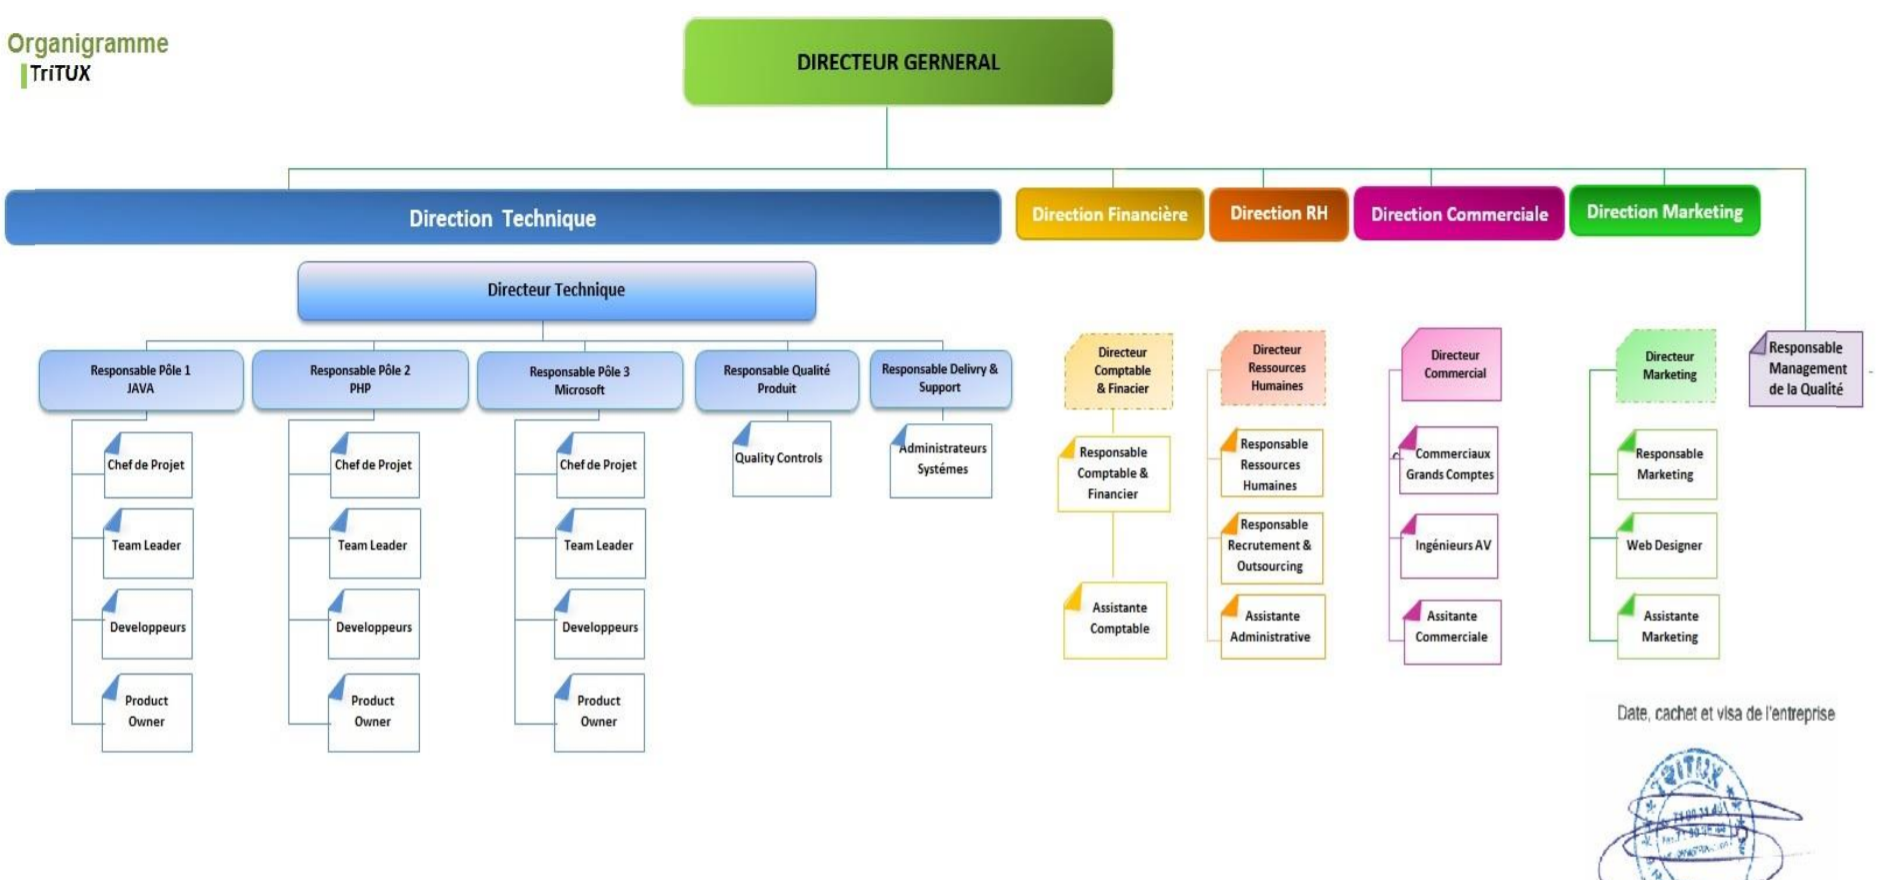
\includegraphics[width=18cm]{organigramme.PNG}
	\caption{Organigramme de TRITUX}
	\label{Organigramme de TRITUX}
\end{figure}
\newpage
\section {Cadre du projet}
\subsection{Contexte du projet}
Dans  le  cadre  de  l'optimisation  de  consommation  de  ses  ressources  et  la  diminution  de 
ses  dépenses,  Tritux  vise  à  mettre  en  place  une  plateforme  de  budgétisation  des  ressources 
Cloud.  Pour  ce  fait,  l'entreprise  d'accueil  nous  a  confié cette  tâche  de  conception  et 
développement  d'une  application  de  gestion  des  ressources  Cloud  par 
projet  et  budget. 



\subsection{Problématique}
Avant l'utilisation du Cloud les entreprises ont beaucoup souffert de la complexité de la gestion de leurs systèmes informatiques. Quelle que soit la taille de l'entreprise, elle avait toujours besoin d'investir sur le matériel, sur son installation et sa maintenance afin d'offrir un produit de qualité et de s'imposer sur le marché. Ce qui traduit la migration immense des architectures traditionnelles vers le Cloud.\\Bien que l'utilisation du Cloud renforce la scalabilité de l'entreprise à moindre coût et améliore sa rentabilité. La mauvaise utilisation des ressources provoque des coûts imprévisibles. Ceci s'explique par le fait que le Cloud suit un modèle de payement à l'usage et que
la  quantité  de  ressources  consommées est plus  onéreuse
.\\ À  cet  égard, 
Tritux  est  présenté  comme  étant  l'une  des  entreprises  qui  souffrent  du  surcoût  de consommation 
due à une utilisation  incontrôlée des machines virtuelles(VM). Elle cherche donc à planifier et restreindre l'utilisation 
des  instances  de  VMs  en se basant sur  le budget affecté à chaque  projet ainsi que le rôle et les permissions de chaque employé membre du projet récemment énuméré. 
\subsection{Etude de l'existant}
L'étude approfondie de la politique actuellement utilisée par l'entreprise d'accueil pour la gestion des ressources Cloud présente une phase indispensable pour la réussite de notre travail.
Dans cette section,  nous allons présenter  
la  solution  actuelle  adoptée  par  Tritux pour  gérer  ses  ressources Cloud . Nous allons critiquer cette solution afin d'envisager les points faibles et développer une application qui répond aux besoins de l'entreprise d'accueil.
\subsubsection{Solution actuelle}
Pour orchestrer le fonctionnement des instances de VM et minimiser leurs consommations, TRITUX a utilisé la console de la plateforme de Google Cloud en y intégrant un libellé qui permet d'introduire la durée d'allocation de la machine virtuelle. Dès qu'active, la facturation est donc à l'usage, pendant la durée sollicitée.
\subsubsection{Critiques de l'existant}
Après avoir exposé la  directive adopté par TRITUX pour la gestion de ces instances,  nous  avons  énumérer  quelques limites pour l'adoption de cette solution.Tout  d'abord,  l'utilisation  directe  de  la  console  de  la  plateforme  de  google  Cloud  n'en- 
gendre pas vraiment l'économie de l'argent. En fait , oublier une VM active hors échéance 
épuise rapidement et sans intérêt la durée sollicité. L'entreprise se trouve obligé d'étaler cette durée pour assurer l'avancement du projet. Ceci provoque  des  frais  supplémentaires .  Ensuite,  la  plateforme  de  Google  Cloud  ne  permet 
pas  de  restreindre  la gestion  des  VMs  par  privilège. En d'autre terme, elle n'a aucune vision sur les projets ni sur les rôles des membres. Elle active et désactive les instances suite à des requêtes émises par l'entreprise.  Ainsi  cette  dernière,  n'offre pas les  fonctionnalités  suivantes: 
: \begin{itemize}
	\item Authentification sécurisé et gestion d'accès ( compte employé, oublie mot de passe,etc).
	\item Affectation des  instance  de  VM  à  un  projet bien spécifique. .
	\item Contrôle de budget  du  projet  .
	\item Gestion  des  employés (profil, rôle,etc).
	\item Restriction d'accès  aux  projets  et  aux instances  de  VMs.
\end{itemize}

\subsubsection{Objectifs du projet }
Après avoir dégagé  
les  problèmes du système existant , l'entreprise d'accueil nous a proposé dans le cadre de notre projet de fin d'étude de  concevoir  et d' implémenter  une  application  de  gestion  des  ressources 
Cloud par projet et budget. Pour ce faire, la manipulation et  l'intégration des APIs  du 
fournisseur Google Cloud platform constitue la base de notre projet. Ces API  répondent aux besoins d'automatisation de fonctionnement des machines virtuelles basée  sur des critères de décisions. Parmi ces critères nous développons un planificateur  
de temps et de budget afin 
d'empêcher l'utilisation anarchique des instances.
 Nous visons aussi à intégrer d'autres modules qui facilitent l'utilisation de notre application. Nous citons: 
 \begin{itemize}
 	\item 	Module d'authentification et de gestion de compte utilisateur:
 	\item 	Module de gestion des utilisateurs.
 	\item 	Module de gestion de projet.
 	\item 	Module de création des machines virtuelles: permet de se débarrasser de l'obligation de la création des VMs à partir de l'interface du fournisseur 
 	
 \end{itemize}

\section{Etat de l'art}
Dans  cette  partie,  nous  allons  présenter  et  analyser en premier lieu les  solutions  existantes  dans  le 
marché. En second lieu, nous allons définir les notions de base indispensable à la compréhension de à notre projet notamment  la  virtualisation et le  Cloud 
Computing. Nous allons présenter en dernier lieu le  fournisseur de service Cloud avec lequel collabore l'entreprise d'acceuil  et les  services  qu'on  va  utiliser. 


\subsection{Analyse et critique des solutions existantes dans le marché}
Dans  cette  section,  nous  présentons  une  analyse  des  solutions  de  surveillance  et  de 
gestion  des  instances  de  machine  virtuelle  (VM).  Ces  applications  ont  pour  but  de 
démarrer/arrêter  les  VM,s  , de  surveiller  leurs  états  et  leurs  performances  et  de  planifier 
leurs  fonctionnements.
Nous citons : 
\begin{itemize}
	\item CloudCheckr.
	\item Skeddly.
	\item ParkMyCloud.
\end{itemize}
Le tableau 1.2 ci-dessous souligne une analyse comparative des fonctionnalités de ces solutions.
\begin{table}[H]
	
	\caption{Etude comparative des solutions existantes dans le marché}
	\label{Etude comparative des solutions existantes dans le marché}
	
	\begin{tabular}{|p{2.8cm}|p{6.2cm}|p{5.7cm}|}
		\hline
		\textbf{Applications} & \textbf{Points forts}& \textbf{Limites}\\
		\hline
		\textbf{ParkMyCloud} & \begin{itemize}
			\item Réduction du  coût de la VM par le contrôle et la planification des ressources.
			\item  Contrôle d'accès et de permissions à travers les structures d'équipes et les rôles. 
			
		\end{itemize}         
		& \begin{itemize}
			\item Manque de possibilité d'ajout de nouvelles instances Cloud directement à partir de la plateforme.
			\item Gestion des instances guidée par le temps uniquement.
		\end{itemize}\\    
		\hline
		\textbf{Skeddly} & \begin{itemize}
			\item Simplicité d'utilisation offre aux clients une gestion guidées des services Cloud.
			\item Prix abordable pour les petites  et moyennes entreprises. 
			
		\end{itemize}         
		& \begin{itemize}
			\item Dépendance aux ressources Cloud d'Amazon uniquement.
			\item Manque de l'analyse de capacité qui permet d'optimiser  la performance et l'efficacité des ressources existantes.
		\end{itemize}\\    
		\hline
		\textbf{CloudChekr} & \begin{itemize}
			\item Respect d'engagement de services par le "Service level agreement" (SLA).
			\item  Documentation automatisée des logs.
			\item  Identification proactive des risques pour gérer la sécurité du Cloud public. 
			\item Analyses de facturation détaillées avec des alertes.
			
		\end{itemize}         
		& \begin{itemize}
			\item Interface utilisateur complexe.
			\item Quelques fonctionnalités ont tendance à se rompre sans avertissement.
			\item Coût relativement cher.
		\end{itemize}\\    
		\hline
	\end{tabular}
\end{table}
Comme  l'illustre  le  tableau  1.2,  ces  applications  sont  bien  riches  en  fonctionnalités 
intéressantes.  Cependant,  Tritux  n'a  pas  adopté  l'une  de  ces  plateformes   vu  que 
certaines  fonctionnalités  ne  sont  pas  conformes  aux  besoins  de  l'entreprise. Parmi les frein de l'adoption nous citons :  

\begin{itemize}
	\item  Allocations des instances  de  VMs  non  budgétisées. 
	\item  Solution pour  Multi-cloud  Cloud  or  Tritux  coopère  avec un unique  fournisseur.
	\item  Grande  quantité  de  données  qui  rend  l'utilisation  de  plateforme  difficile et lourde. 
	\item  Inaptitude  à  créer  des  instances  du  fournisseur  Cloud  via  la  plateforme. 
	\item Une inaptitude à créer des instances du fournisseur Cloud via la plateforme.
	\item Solutions payantes.
	\item Absence de gestion des projets.
\end{itemize}


\subsection{Virtualisation}

Toute entreprise cherche à améliorer l'efficacité et la disponibilité de ses ressources.  Elle cherche à remplacer  
l'ancien  modèle  "un  serveur dédié pour une  application" par  « un serveur dédié à plusieurs applications »  grâce à la  virtualisation.
Du coup, la virtualisation a  entamé  le  monde 
de  l'informatique  avec  beaucoup  plus  d'avantages  tels  que  : 
\begin{itemize}
	\item Utilisation optimale des ressources.
	\item Allocation dynamique de la puissance de calcul en fonction des besoins.
	\item Economie sur le matériel par mutualisation.
\end{itemize}



Selon Redhat « La virtualisation est une technologie qui permet de créer plusieurs environnements simulés ou ressources dédiées à partir d'un seul système physique. Son logiciel, appelé hyperviseur, est directement relié au matériel et permet de fragmenter ce système unique en plusieurs environnements sécurisés distincts. C'est ce que l'on appelle les machines virtuelles, ou VM. Ces dernières exploitent la capacité de l'hyperviseur à séparer les ressources du matériel et à les distribuer convenablement. »[redhat]. \\
:  Il existe plusieurs  types de virtualisation parmis lesquels nous citons :
\begin{itemize}
	\item \textbf{Virtualisation matérielle}: Le type de virtualisation le plus courant L'hyperviseur crée des versions virtuelles des ordinateurs et des systèmes d'exploitation et les consolide en un seul grand serveur physique.
	\item \textbf{Virtualisation du serveur}:  Un regroupement des serveurs physiques sous-employés sur un seul hôte  qui exécute des systèmes virtuels.
	\item \textbf{Virtualisation du stockage}: Une virtualisation économique permettant de regrouper un ensemble  de périphériques de stockage afin qu'il rassemble à un seul périphérique.
	\item \textbf{Virtualisation du système d'exploitation}: Le noyau autorise l'existence de plusieurs instances d'espaces utilisateurs, cette virtualisation est utilisée principalement pour tester les applications sur différentes plateformes de système d'exploitation.
\end{itemize}
La virtualisation et le cloud computing sont deus notions complémentaires. Ceci s'explique par le fait que la délivrance des services Cloud se repose principalement sur la virtualisation.  Le Cloud Computing n'est pas donc une invention mais une évolution des technologies. Nous allons exposer dans la section suivante ce nouveau paradigme.
\subsection{Cloud Computing}
De  plus  en  plus  utilisé,  le  cloud  computing  est  jusqu'à  présent  considéré  comme  l'évolution  majeure  de  l'informatique  du  21ème  siècle.  Ce  dernier  est  devenu  la  fourniture  des 
services  informatiques,  permettant  un  accès  omni présent ,à  la  demande, à traves un réseau   
à  un  pool  de  ressources  informatiques partagé. Cet accés obéit à la règle n' importe où n'importe quand et n'importe comment. 
 Ces ressources peuvent être des applications,  puissances de calcul, espaces de stockage  ou serveurs indépendamment de leurs localisations géographiques.\\
Pour réussir à présenter une innovation et un meilleur produit à leurs clients, Les grandes entreprises du  secteur informatique sont massivement impliquées dans des activités liées au Cloud en faveur de profiter de ses services. \\
En se basant sur une couche d'abstraction  proposée par la virtualisation. Cloud Computing offre trois types de services définies par la figure 1.2. 
\begin{figure}[ht]
	\centering
	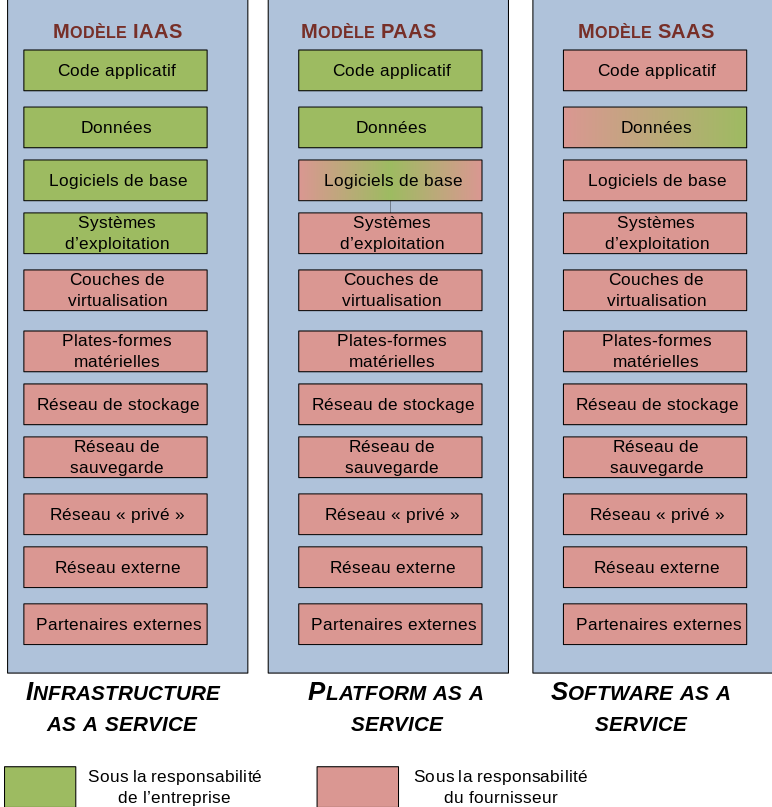
\includegraphics[scale=0.7]{servicesCloud.jpg}
	\caption{Les services du Cloud Computing}
	\label{Les services du Cloud Computing}
\end{figure}
\begin{itemize}
	\item   \textbf{Software-as-a-service} (SAAS): Des applications, aux abonnements, installées ou accessibles via un navigateur. En profitant de ce type de service les fournisseurs gèrent de manière transparente l'ensemble des aspects techniques de l'application. Quant aux clients, ils se limitent à effectuer quelques paramétrages de l'application. 
	\item \textbf{Plateform-as-a-service} (PAAS): Des plateformes de développement ou de test dont le système d'exploitation et les outils sont gérés par les fournisseurs du Cloud. Or les clients gardent la main sur l'installation des applications et leurs paramétrages.
	\item   \textbf{Infrastucture-as-a-service} (IAAS): Les fournisseurs offrent des ressources informatiques  virtualisées (stockage, réseaux, virtualisation, etc.) sur lesquelles le consommateur garde le contrôle sur le système d'exploitation, les applications déployées  et certains composants de réseau. 	Les domaines d'exploitation des infrastructures sont divers, Ils peuvent être  utilisées  comme un réseau privé virtuel dans les entreprises ou pour héberger des sites sur des serveurs virtuels ou pour l'utilisation des data centers virtuels. 
	
\end{itemize}
Ces services peuvent être déployer sur différents modes : \begin{itemize}
	\item \textbf{Cloud privé} : C'est un modèle très répandu dédié à une seule entreprise. Le déploiement de ce dernier peut se faire sous deux autres formats possibles:
	\begin{itemize}
		\item {Cloud privé internalisé}: Dans ce cas, le Cloud est interne à l'entreprise ou entièrement dédié à cette même entreprise. Il est accessible via des réseaux sécurisés et opérés par les équipes internes.
		\item {Cloud privé externalisé}: Dans ce cas, le Cloud offre des services similaires au Cloud privé internalisé. Ce dernier est entièrement dédié à l'entreprise, mais hébergé chez un tiers.
	\end{itemize}
	\item \textbf{Cloud public}: Dans ce cas, le Cloud est externe à l'entreprise et géré par un opérateur externe propriétaire des infrastructures, avec des ressources totalement partagées entre tous ses clients.
	\item \textbf{Cloud hybride}: Dans ce cas, il s'agit de l'association de deux ou plusieurs modèles de cloud pour assurer une portabilité des applications et des données.
\end{itemize}
Bien que le marché du Cloud public est plein de fournisseurs, la concurrence est toujours concentrée entre Amazaon Web Services, Microsoft Azure et Google Cloud Plateform. 
Pour des raisons d'efficacité et de disponibilité, le choix de fournisseur pour Tritux a été fixé sur Google Cloud Plateform.
\subsection{Google Cloud plateform}
La plateforme Cloud de Google (GCP) est un ensemble de ressources informatiques, mises à la disposition du grand public via des services modulaires basés sur le Cloud, sous la forme d'une offre de cloud public.\\
Celle-ci propose des services de calcul, stockage, apprentissage automatique et d'internet des objets, ainsi que des outils de gestion et de sécurité. Les principaux produits de Cloud computing de Google Cloud Platform sont répartis en trois grandes familles:
\begin{itemize}
	\item \textbf{Google App Engine}:  Un  service  Cloud  de  type  PAAS  permet  aux  développeurs 
	d'accéder  à  l'hébergement  évolutif  de  Google.  Les  développeurs  peuvent  également 
	utiliser  un  kit  de  développement  logiciel  pour  implémenter  des  produits  logiciels 
	s'exécutant  sur  App  Engine. 
	\item \textbf{Google Storage}:Une  plateforme  de  stockage   conçue  pour  stocker  des 
	Données de taille importante.
	
	\item \textbf{Google Compute Engine}: Une offre IaaS qui permet aux clients d'exécuter des charges de travail sur le matériel physique de Google.
Il fournit un nombre évolutif de machines virtuelles (VM) pouvant servir de grands clusters de calcul à cette fin.  Google Compute Engine peut être géré via une API REST, une interface de ligne de commande (CLI) ou une console Web. Compute Engine est un service à la carte avec un minimum de 10 minutes.\\
Ainsi ces ressources virtuelles devront être  instanciées, allouées et orchestrées via des plateformes d'administration et de gestion des ressources Cloud.
\end{itemize}

\section{Méthodologie de gestion de  travail }
Dans le processus de réalisation d'un projet complexe, l'utilisation d'une méthodologie de 
management  de  projet  est  indispensable  afin  d'assurer  la  réussite  de  ce  dernier.  En  e?et, 
une  bonne  méthodologie  de  projet  fournit  le  cadre,  les  procédés,  les  lignes  directrices  et 
les  techniques  pour  gérer  à  la  fois  le personnel  et  le  travail. 
.\newline
Il existe  de  nombreuses  méthodologies  de  gestion  de  projet,  assez  différente  les  unes  des 
autres  de  par  leurs  fonctionnements,  mais  ils  se  rejoignent  tous  afin  de  garantir  le  succès 
de  la  conduite  du  projet. \newline
Pour notre projet nous avons opté pour une méthode agile qui permet de se focaliser sur la valeur métier du livrable, d'améliorer constamment la qualité de ce que nous réalisons et de réagir efficacement aux changements.
De ce fait, nous allons donner tout d'abord un aperçu sur les méthodologies agiles. Puis, nous focalisons sur la méthodologie Scrum, qui a été utilisée dans le présent projet.
\subsection{Méthodes Agiles}
Les besoins, dans une équipe de développement logiciel qui travaille sur un projet interne sont parfois susceptibles d'être changés ou modifiés. De ce fait, l'équipe se trouve
en train de développer une application avec des spécifications parfois non précises, ce qui
peut entraîner des retards dans le déploiement du projet. Ces problématiques ont poussé
les ingénieurs à réinventer les méthodes de gestion de projet et de conception en introduisant ce que nous appelons la méthode Agile.
\subsection{Presentation de la méthodologie Scrum}
Scrum est la méthodologie suivie par la société TRITUX pour la gestion de ses projets. C'est une méthodologie agile itérative basée sur des itérations d'une durée de 2 à 4 semaines appelées Sprints.
Durant chacune de ces itérations, une partie du produit nommée .« Incrément » est réalisée en se basant sur les parties crées lors des itérations précédentes et livrées à la fin du Sprint.

Elle  offre les avantages suivants : \begin{itemize}
	\item Flexibilité. 
	\item Pas de distinction des rôles au sein d'une équipe « Scrum ». 
	\item Auto confiance au sein de l'équipe en l'isolant durant le Sprint et en la rendant autogérée. 
	\item Équipes soudées. 
	
\end{itemize}

Il existe différents rôles participants dans la mise en \oe{}uvre

 du projet selon la logique de Scrum: 
\begin{itemize}
	\item \textbf {Product Owner } : C'est un membre à part entière de l'équipe Scrum dont la responsabilité principale est de définir un produit qui apportera le maximum de valeur métier aux utilisateurs dans le temps et le budget. Il présente les besoins du client et propose de nouveaux objectifs. Il contrôle aussi la qualité et la date de délivrance de chaque sprint 
	\item \textbf  {Scrum Master }: Il aide  l'équipe à travailler de façon autonome et à s'améliorer constamment. Il est le garant de l'application du processus, Scrum en l'occurrence. 
	\item \textbf { Scrum Team}: L'équipe de développement 
\end{itemize}

Les artéfacts de cette méthodologie sont de deux types: \cite {ref3}

	\begin{enumerate}
		\item \textbf {Backlog produit }: liste ordonnée de tout ce qui pourrait être requis dans le produit et elle est l'unique source des besoins pour tous les changements à effectuer sur le produit sous la responsabilité du Product Owner. 
			\item \textbf {Backlog sprint }: est constitué à partir des thèmes du Backlog produit. Lors de la réunion de planification de sprint, l'équipe de développement choisit les éléments du Backlog produit qui seront réalisés. Il est sous la responsabilité de l'équipe et elle est seule à pouvoir le modifier en cours d'itération. 
	\end{enumerate}



\section{Conclusion}
 Ce chapitre nous a permis d'introduire notre projet, de présenter l'organisme d'accueil  et  la problématique qui nous suscite à la réalisation de ce projet, ainsi que la solution proposée. Notre rapport sera organisé en respectant les normes de la méthode Agile SCRUM.
En vue de mieux comprendre le métier, une description de l'environnement fera l'objet
du prochain chapitre.
